\chapter{Overview of the Cosmos SDK}
\label{OCS:overview}
The Cosmos SDK architecture, its modules and functionalities will all be covered in-depth in this chapter. Highlighting the advantages of using the Cosmos SDK for blockchain development alongside the challenges that developers may encounter when implementing the framework.

\section{High-level Overview}
The Cosmos SDK is an open-source framework for creating both permissioned \gls{poa} blockchains, like the Cosmos Hub\cite{cosmos-hub}, and multi-asset public \gls{pos} blockchains. Application specific blockchain is a widely used term for blockchains developed using the Cosmos SDK.

Compared to virtual machine blockchains, application specific blockchains offer a fundamentally different development paradigm. Developers are completely free to make the architectural choices necessary for an application to function efficiently on a blockchain that has been specifically created to run a single use case, as shown in Lst~\ref{lst:app-based-blockchain}. Moreover, they can offer greater performance, security, and sovereignty.

\newpage
\begin{lstlisting}[language=bash, caption=Application based blockchains. Source:\cite{app-based-blockchain},label={lst:app-based-blockchain}]
                ^  +-------------------------------+  ^
                |  |                               |  |   Cosmos SDK
                |  |  State-machine = Application  |  |
                |  |                               |  v
                |  +-------------------------------+
                |  |                               |  ^
Blockchain node |  |           Consensus           |  |
                |  |                               |  |
                |  +-------------------------------+  |   CometBFT
                |  |                               |  |
                |  |           Networking          |  |
                |  |                               |  |
                v  +-------------------------------+  v
\end{lstlisting}

\section{Architecture}
A blockchain is essentially a replicated deterministic state machine. When a state S and a transaction T are provided, the state machine will produce a new state S', as seen in Lst \ref{lst:state-transition}.

\begin{lstlisting}[language=bash, caption=State machine transition. Source:\cite{app-based-blockchain},label={lst:state-transition}]
                +--------+                 +--------+
                |        |                 |        |
                |   S    +---------------->+   S'   |
                |        |    apply(T)     |        |
                +--------+                 +--------+
\end{lstlisting}

The transactions are actually grouped together in blocks to improve process efficiency. The state machine will produce a new state S' from a state S and a block of transactions B, as seen in Lst \ref{lst:state-block-transition}.
\newpage
\begin{lstlisting}[language=bash, caption=Block of bundled transactions. Source:\cite{app-based-blockchain},label={lst:state-block-transition}]
            +--------+                              +--------+
            |        |                              |        |
            |   S    +----------------------------> |   S'   |
            |        |   For each T in B: apply(T)  |        |
            +--------+                              +--------+
\end{lstlisting}

With the Cosmos SDK, developers have a great range of flexibility to define the state of their applications, transaction types, and state transition processes. The next sections provide a more thorough explanation of how to build state machines using the Cosmos SDK. Let's first analyse how CometBFT operates to replicate the state machine.

\subsection{CometBFT}

The networking and consensus layers of a blockchain are handled by the application agnostic engine CometBFT, as seen on Lst~\ref{lst:app-based-blockchain}. CometBFT is responsible for sorting and propagating transaction bytes. This engine relies on the \gls{bft} algorithm developed by Tendermint to reach consensus.

Validators are a group of unique nodes that the CometBFT consensus algorithm uses. The blockchain is updated with new blocks of transactions by validators. A validator set V is present at any given block. The process selects a validator in V to be the next block's proposer. If more than two thirds of V signed a prevote and a precommit on it, and if all the transactions it contains are genuine, this block is regarded as genuine. Rules defined in the state machine can alter the validator set. The algorithm follows a simple state machine as shown in Fig\ref{fig:cometbft-overview}.

\begin{figure}[H]
    \centering
    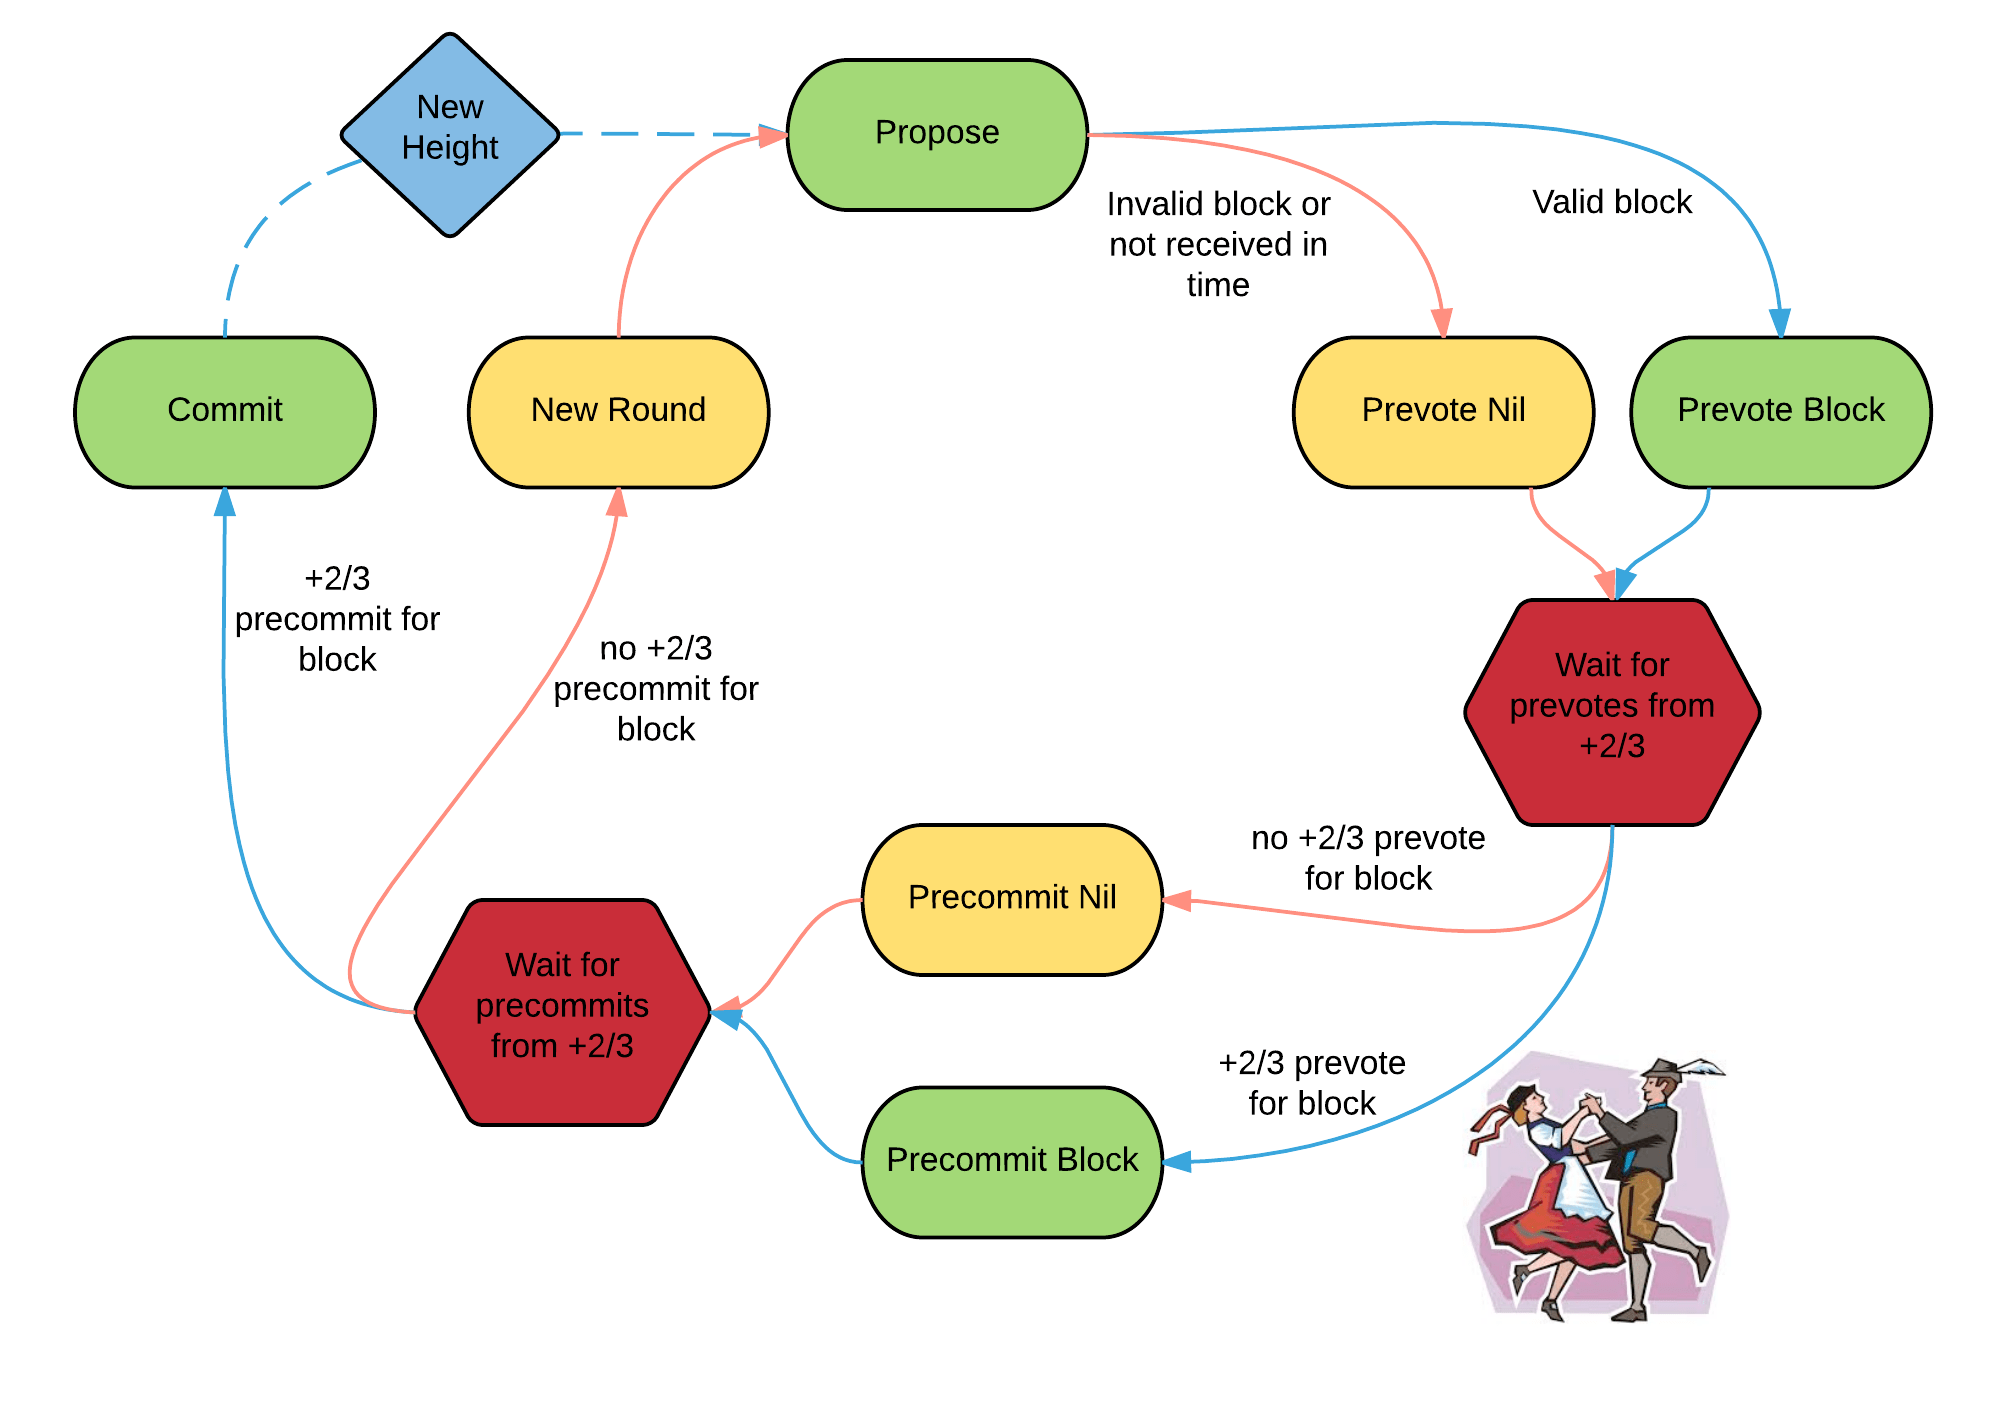
\includegraphics[width=\textwidth]{figures/cometbft.png}
    \caption{Consensus Overview CometBFT Source\cite{cometbft-overview}}
    \label{fig:cometbft-overview}
\end{figure}


\subsection{ABCI}
The \gls{abci} interface is a set of standard protocols that defines the communication between the consensus engine and the application. By enabling the division of consensus engine logic from application logic, it facilitates the development of applications on top of the Cosmos SDK.

The consensus engine and the application can communicate with one another without having to be aware of each other's internal workings thanks to the \gls{abci} interface, which serves as a mediator between them as shown in Lst \ref{lst:ABCI}. The development process is more flexible thanks to this separation of concerns as developers can focus on developing their particular application logic without worrying about the underlying consensus engine. Additionally, because the \gls{abci} interface offers a standardised method for the consensus engine to connect with the application, it facilitates interoperability between various blockchains that make use of the Cosmos SDK.

\newpage
\begin{lstlisting}[language=bash, caption=ABCI Interface. Source:\cite{app-based-blockchain},label={lst:ABCI}]
                      +---------------------+
                      |                     |
                      |     Application     |
                      |                     |
                      +--------+---+--------+
                               ^   |
                               |   | ABCI
                               |   v
                      +--------+---+--------+
                      |                     |
                      |                     |
                      |       CometBFT      |
                      |                     |
                      |                     |
                      +---------------------+
\end{lstlisting}


\section{Applications Architecture}
\label{ch:applicatoins-architecture}

So far this in this chapter we have seen a general overview on how the Cosmos SDK works and why its modular decoupled architecture helps developers when creating their applications. Thanks to CometBFT, developers can focus on the application's logic without having to worry about the uderlaying consensus and communication process of the state machine. In this subsection we will dissect how the application layer of our architecture works.

In fact, the application layer works in a very simple and modular way thanks to the Cosmos SDK. The framework provides us with a simple boilerplate implementation called baseApp. This baseApp implements the necessary methods to route the transactions to the different modules and also implements the \gls{abci} methods to communicate with the cometBTF engine. Modules can be viewed as small state machines within the state machine. They generally define a subset of the state, as well as a subset of message types. These messages are routed by the BaseApp and the module parses them using protobuf definitions. This is how byte transactions handled by the cometBFT are translated into the application logic.

On top of this core, the Cosmos SDK enables developers to build custom modules that implement the business logic of their application. In other words, while the core handles wiring and permits module composition, SDK custom made modules implement the majority of the application's functionality. Fig \ref{fig:application-modules} shows the general architecture of the application layer.

\begin{figure}[H]
    \centering
    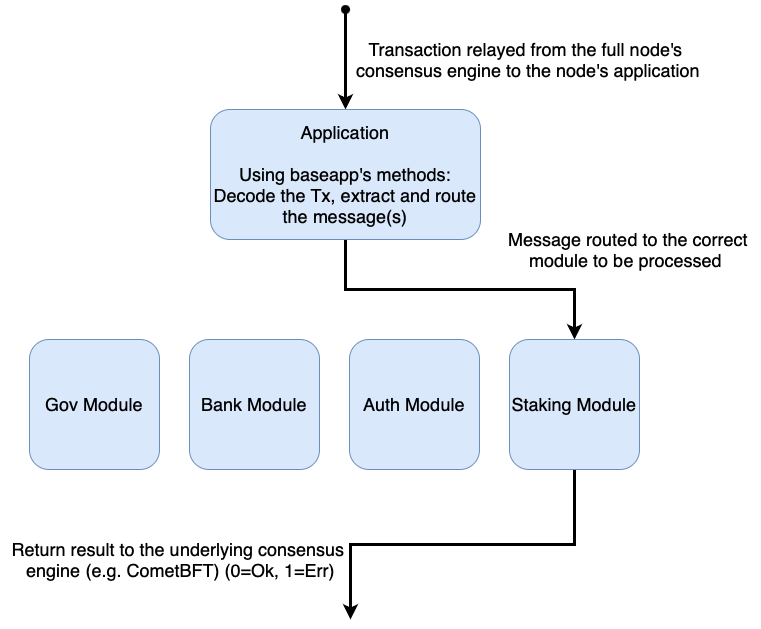
\includegraphics[width=\textwidth]{figures/prueba.png}
    \caption{Application architecture}
    \label{fig:application-modules}
\end{figure}
